\section{Dataset}
\label{sec:dataset}

\begin{figure}[!t]
\label{fig:dataset_teaser}
\centering
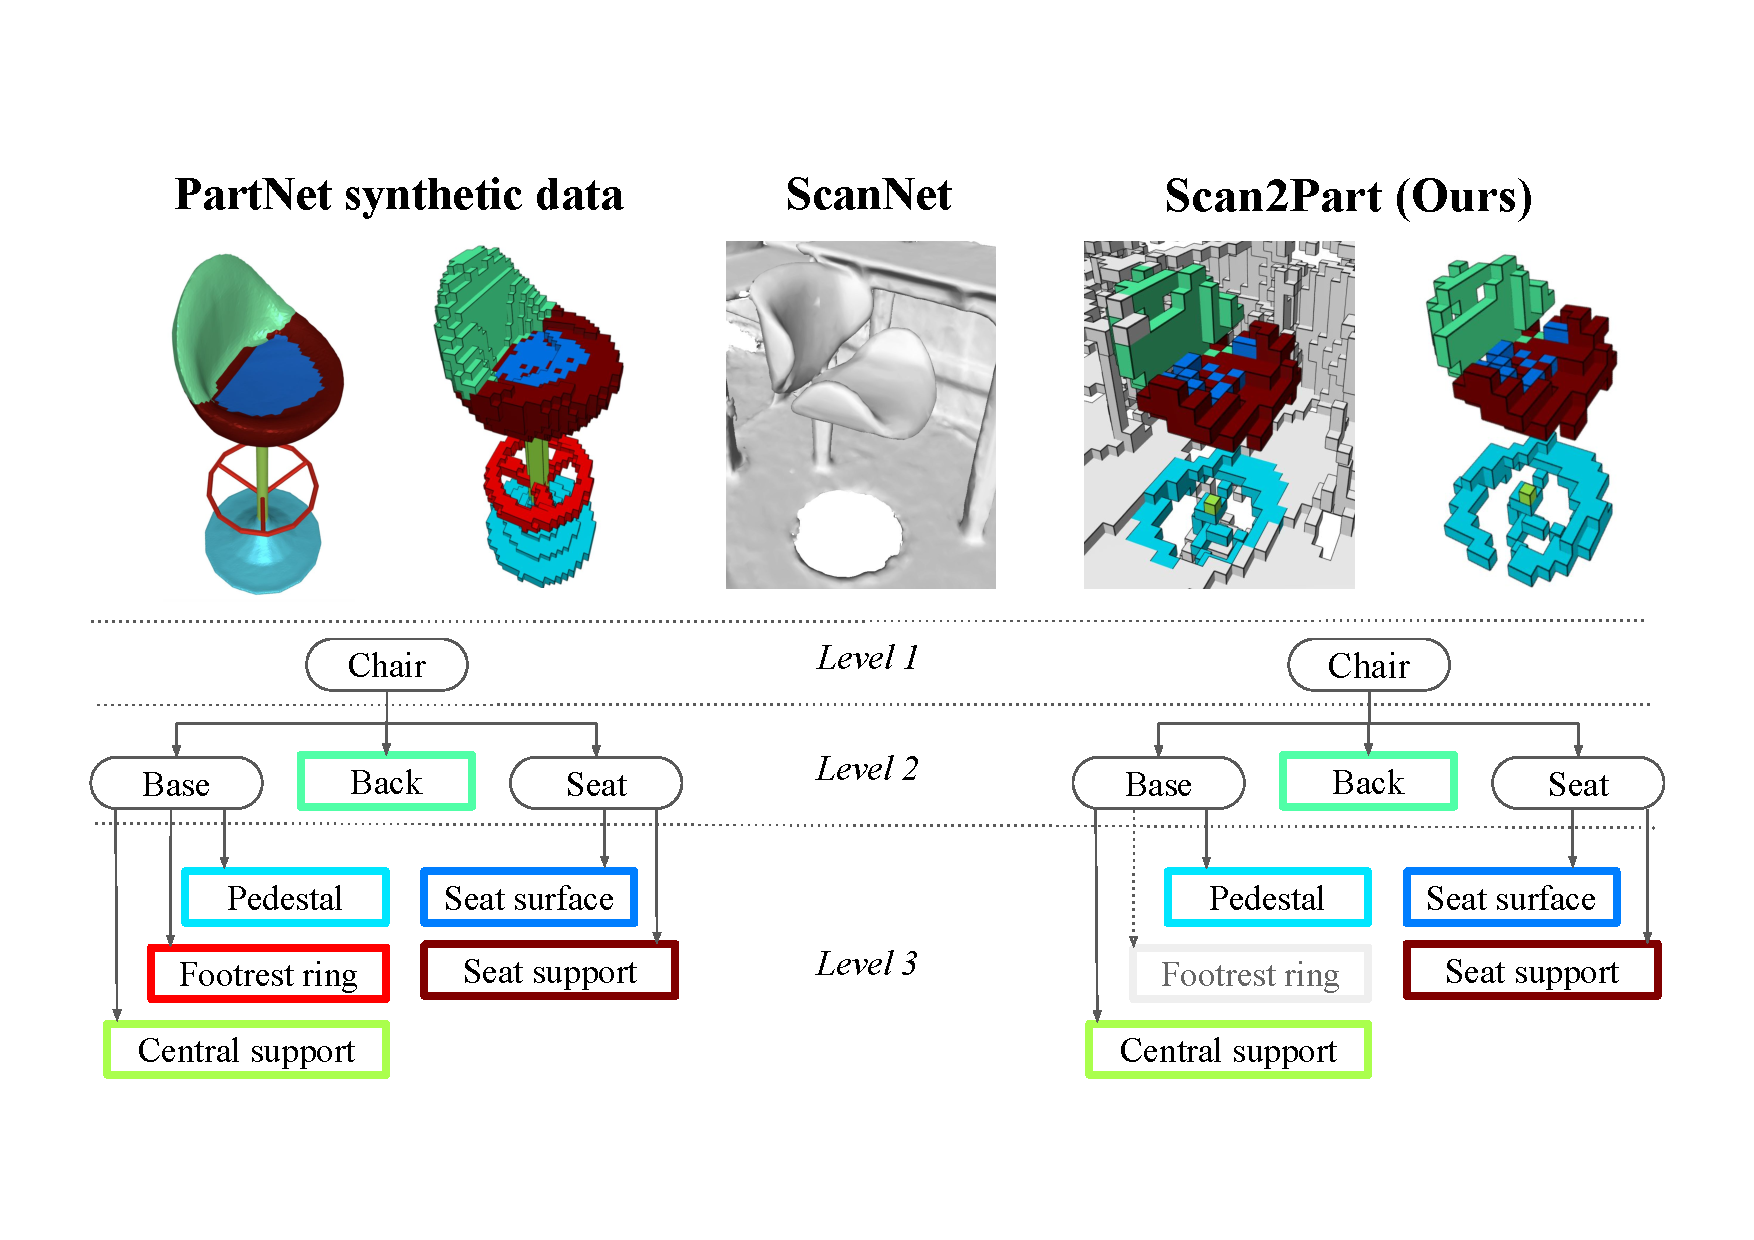
\includegraphics[width=0.99\textwidth]{Figures/scan2part/dataset_teaser.pdf}
\caption{Top:our dataset is obtained by combining PartNet synthetic data with ScanNet sensor data. Bottom: the PartNet object hierarchy is compressed to include only parts sufficiently well represented in ScanNet data.}
\end{figure}

Our first objective is to develop a large-scale 3D scene understanding dataset with part-level annotations. 
We use the 3D geometry in 1,506 3D scenes in ScanNet dataset~\cite{dai2017scannet} reconstructed from RGB-D scans in the form of truncated Signed Distance Function (SDF) at voxel resolution = 3\,cm.
For labeling the scan geometry, we use the parts taxonomy in PartNet dataset~\cite{mo2019partnet} represented as a tree structure where nodes encode parts at various detail levels and edges encode the ``part of'' relationship.
We associate to each 3D scene a per-voxel mask storing leaf part IDs from the taxonomy (i.e., the most fine-grained categories).
To label the 3D scene at a given level~$d$ of semantic detail ($d = 1$ meaning whole objects and $d = 8$ meaning finest parts), we start with the leaf labels in each voxel and traverse the taxonomy tree until hitting depth~$d$.



We further describe the main steps taken to create our Scan2Part benchmark below, leaving the detailed discussion of the technicalities for the supplementary. 
% \DZ{This figure is commented out}
Annotation schema for our dataset is shown in Figure~\ref{fig:dataset_schema}.

\paragraph{Transferring labels to volumetric 3D grids.} 
% \LA{add something about semantic correspondences, ie WHICH object must be where}
To obtain ground-truth semantic parts annotations for real-world 3D scenes, we establish  correspondences between each volume in the 3D scene in ScanNet and a set of part-annotated mesh vertices in a registered 3D CAD model from PartNet.
To this end, we first find accurate 9 degrees of freedom (9\,DoF) transformations between PartNet 3D models and their original versions from ShapeNet, and next use the manually annotated 9\,DoF transformations and their respective object categories provided by Scan2CAD to obtain the final scan-to-part alignments.
We further perform a simple majority voting, selecting only the most frequent (among the vertices) part label as the ground truth voxel label, see Figure~\ref{fig:scan2part_labels_transfer}.
% \LA{how many classes typically fall into this selection and get suppressed in this procedure?}

\begin{figure}[!h]
\label{fig:scan2part_labels_transfer}
\centering
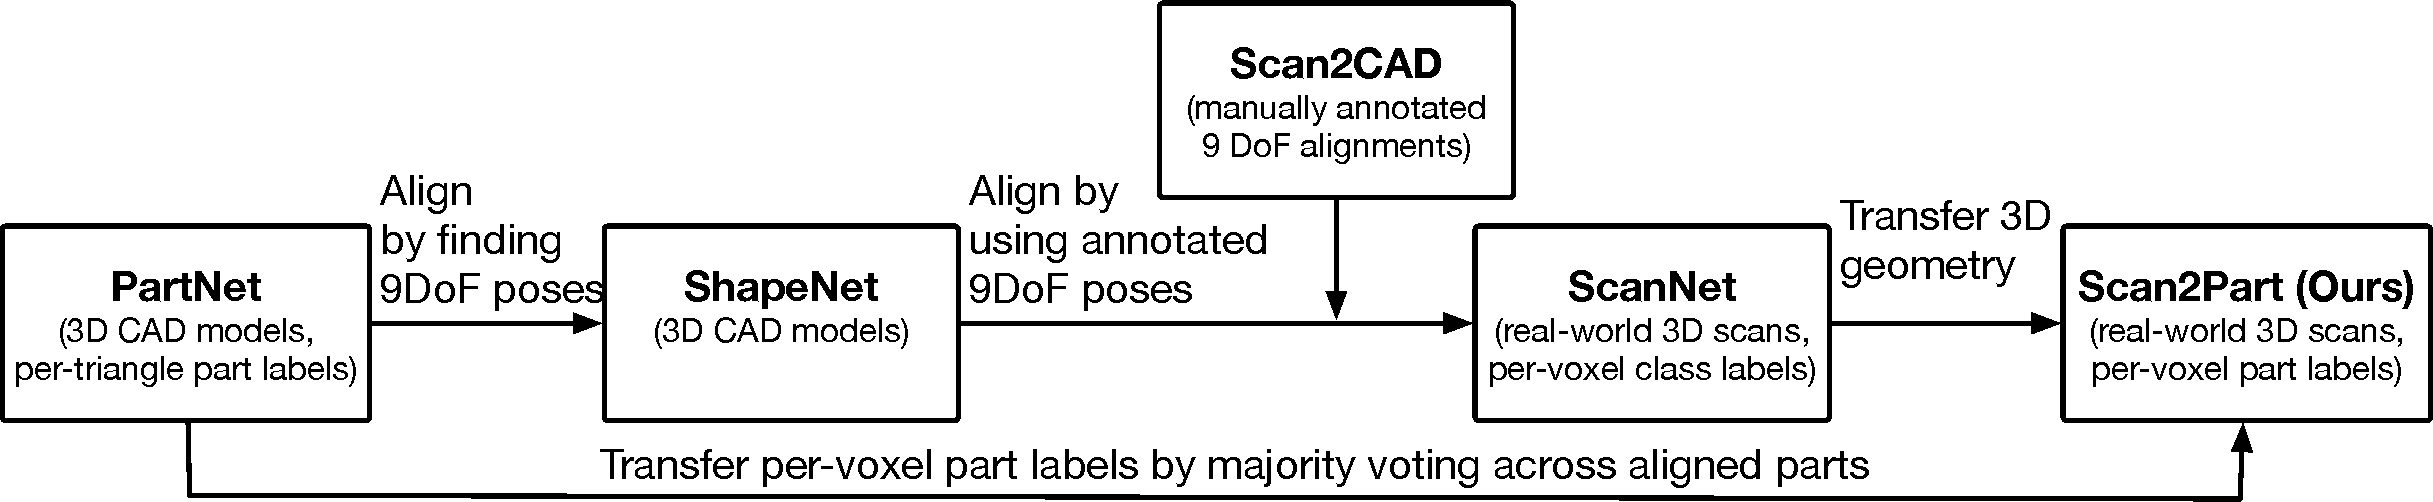
\includegraphics[width=0.99\textwidth]{Figures/scan2part/scan2part_labels_transfer.pdf}
\caption{Our automatic pipeline for part-based 3D scan annotation (see surrounding text).}
\end{figure}


% For this procedure to operate, one needs to register a set of 3D shapes to scans.
% Our resulting Scan2Part dataset consists of

This procedure results in 242,081 correspondences represented as 9\,DoF transformations between 1,506 reconstructions of real-wold ScanNet scenes and 53,618 unique parts of 2,477 ShapeNet objects.
Parts of each object have a tree structure, similar to~\cite{mo2019partnet}.
Note that the majority-based voting implementation of annotation transfer results in some semantic parts labels not being represented in the 3D scan, ultimately affecting parts taxonomy, which we discuss below. 

% we could sample or somehow ensure that at least some representatives of all classes exist in the dataset
% however, we have chosen the simplest implementation in the form of the simple majority voting 
% this results in some classes being omitted due to the finite scan resolution
% in the end, this affects part hierarchy

\begin{figure}[!t]
\label{fig:dataset_schema}
\centering
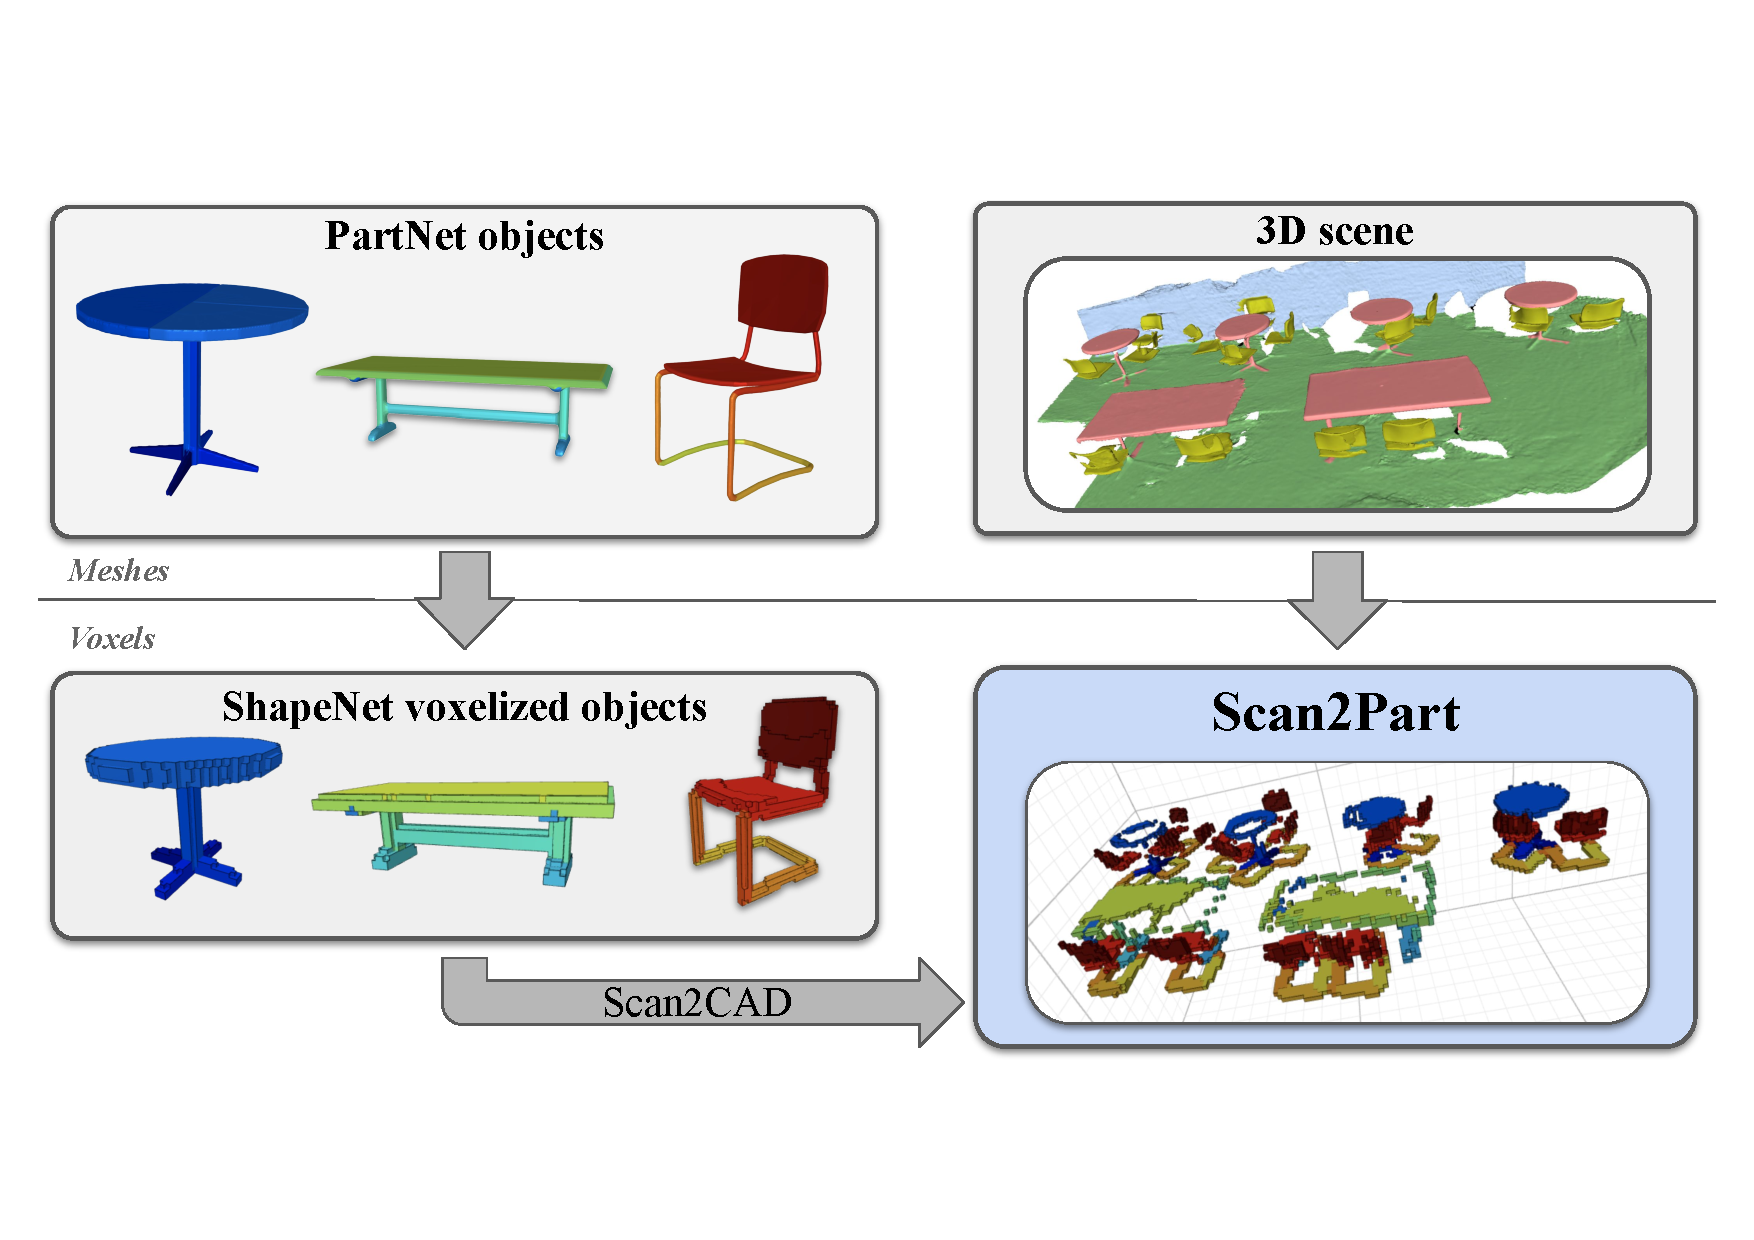
\includegraphics[width=0.9\textwidth]{Figures/scan2part/dataset_schema.pdf}
\caption{A pipeline for obtaining Scan2Part dataset. We project the PartNet \cite{mo2019partnet} labels to the ShapeNet \cite{chang2015shapenet} coordinate system (left), then use Scan2CAD \cite{avetisyan2019scan2cad} dataset to map labels to real scenes from Scannet \cite{dai2017scannet} (right).}
\end{figure}



% \begin{figure}[!t]
% \label{fig:part_level_variation}
% \centering
% 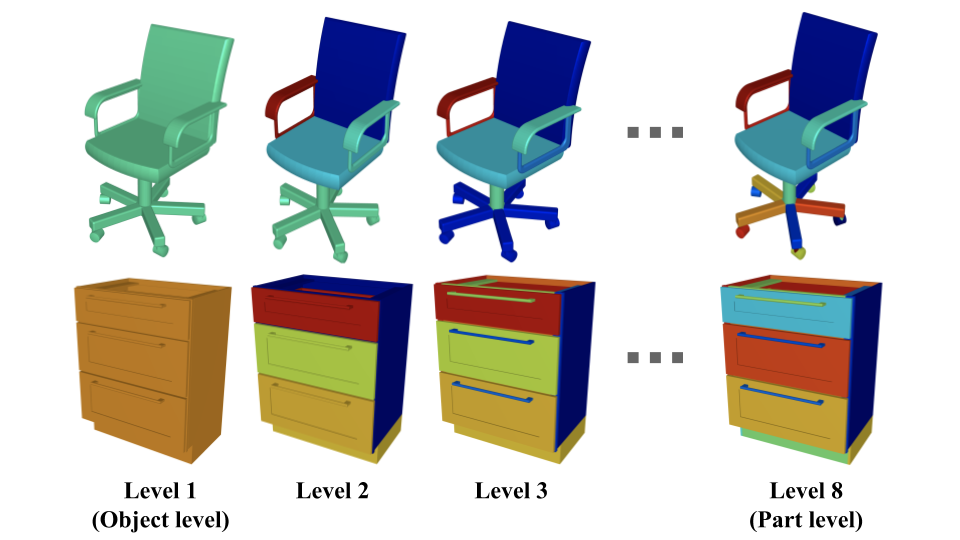
\includegraphics[width=\textwidth]{Figures/scan2part/part_level_variation.png}
% \caption{The object level of detail depending on the part taxonomy tree level based on PartNet taxonomy~\cite{mo2019partnet}. The level of detail  increases from left to right, starting with the object level.}
% \end{figure}

\paragraph{Parts taxonomy processing. } 
% % 1. description of the taxonomy
% % issue: classes that are not represented in 3D scans
% % 2. compressing taxonomy by merging classes
% % 3. compressing taxonomy by pruning the taxonomy tree
% % say something about taxonomy 
The taxonomy of 3D shape parts is represented as a single tree structure based on~\cite{mo2019partnet}. However, as the voxel resolution of the real-world 3D scan is relatively coarse, particular part categories (e.g., small shape details such as keyboard buttons or door handles) cannot be represented by sufficient number of 3D data points, thus implying a reduction in the original taxonomy. 
We proceed with this reduction by first choosing an appropriate occurrence threshold (we pick 1800 voxels, but demonstrate the effect of different threshold values in the supplementary) and remove classes that have smaller number of representatives in the dataset.
% % there are at least 1800 voxels labeled with this part\DZ{why 1800?}  in the entire dataset.
We finalize the taxonomy by pruning trivial paths in the tree (i.e., if a vertex has only one child, then we delete this vertex by connecting the child and the parent of this vertex), but keeping the leaf labels intact. We display the number of vertices at different granularities in the original and resulting part taxonomy levels in Table~\ref{tab:label_presence}.  
Some parts (leafs in the part taxonomy) are not represented in ScanNet data, so we remove these from the tree. 
% At the first tree level, each tree node  represents an entire object (bed, chair, table, etc.), at the second tree level --- the object base components (bed base, soft part, etc.), and so on.  An example of coloring an object by parts for different taxonomy levels is shown in the figure~\ref{fig:part_level_variation}
% %Each tree level is a level of object details: the deeper the tree level, the more detailed the parts division becomes.

% % we project partnet into scannet not vice-versa 
% % one could have done the other way around, e.g. say use subdivision (octrees) and place "ideal" CAD models into the scannet scenes, preserving ALL partnet classes 
% % but we're specifically interested in preserving as much as possible of the scannet noisy geometry 
% % additionally overlap between partnet and scannet categories is lower than 100%

% To build the part taxonomy, we choose the rules for combining the part trees of all the objects represented in Scan2Part. The total number of all instance parts is 242,081, while there are 53,618  unique parts (figure~\ref{fig:three_tables}, left).
% This is an extremely large number of labels for part segmentation, so we have to apply a more intelligent combination of part trees of different objects.
% If we assume that there are identical parts inside the same object, e.g., four table legs are four instances of the ``leg'' part (figure \ref{fig:three_tables}, center), then the total number of unique parts is reduced to 14,782. It is worth noting that in this case, the legs of different tables will be represented as different parts.

% However, if we assume that there are identical parts inside the same object class, i.e. all the legs of all tables are instances of ``leg'' part (figure \ref{fig:three_tables}, right), then the number of unique parts is reduced to 307.  

% % \DZ{It is unclear from the above what the rules actually are. It says if we assume this, then .., and if we assume that, then ...  Please state what exactly the rules are, and then explain why, e.g., to reduce the number of classes (and why this is a good thing)}

% Some parts (leafs in the part taxonomy) are not represented in ScanNet data, so we remove these from the tree. 
% A particular part is considered sufficiently represented if amount of voxels in the entire dataset labeled with this part is above certain threshold. 
% Through analysis of labels distribution we chose our threshold to be equal to 1800 voxels, but demonstrate the effect of different threshold values in the supplementary.
% % there are at least 1800 voxels labeled with this part\DZ{why 1800?}  in the entire dataset.
% After cleaning the tree, we get rid of trivial paths in the tree (if a vertex has only one child, then delete this vertex by connecting the child and the parent of this vertex) \DZ{what happens to labels?}  The number of vertices at different part taxonomy levels is shown in the table \ref{tab:label_presence}. 
% (\textcolor{red}{why do we use the first 3 levels?})

% \begin{figure}[!t]
% \label{fig:three_tables}
% \centering
% 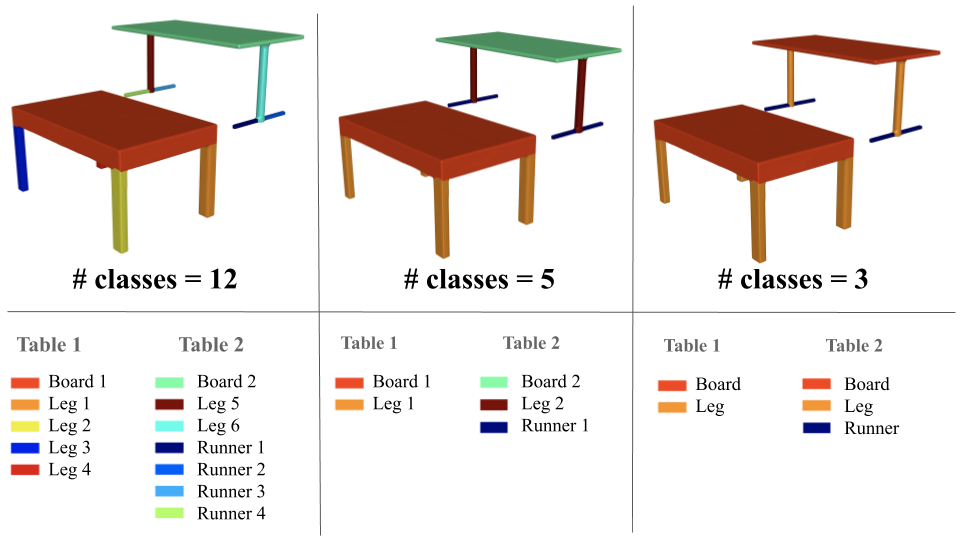
\includegraphics[width=0.9\textwidth]{Figures/scan2part/three_tables}
% \caption{Different rules for combining the part trees of all the objects. \textcolor{red}{TODO}: more specific. (left) if colors of all the legs are different, (center) if color of legs depends on the the table, (right) if color of all legs are the same.}
% \end{figure}


% \begin{figure}[!t]
% \label{fig:three_tables}
% \centering
% 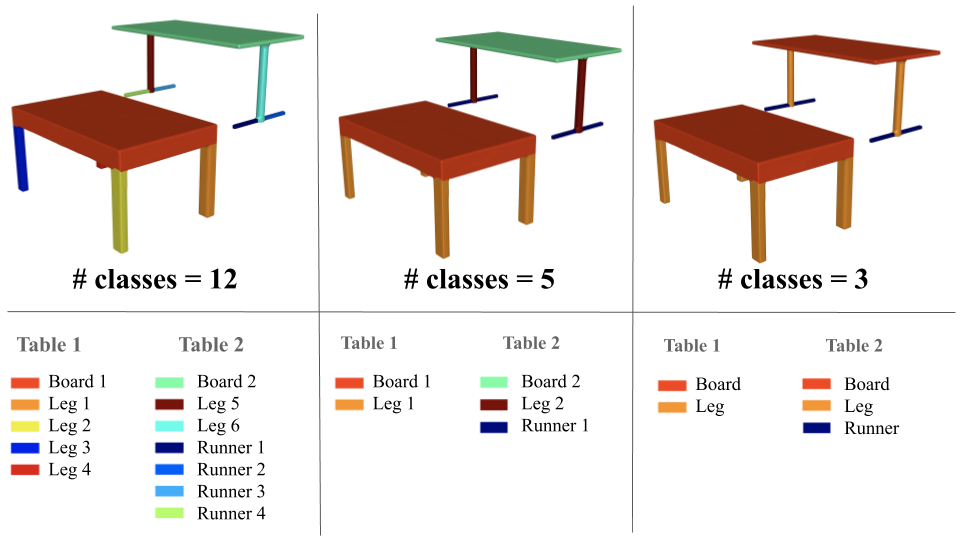
\includegraphics[width=0.9\textwidth]{Figures/scan2part/three_tables}
% \caption{Different rules for combining the part trees of all the objects. \textcolor{red}{TODO}: more specific. (left) if colors of all the legs are different, (center) if color of legs depends on the the table, (right) if color of all legs are the same.}
% \end{figure}





\begin{table}[ht!]
\centering
\caption{Number of parts on each tree level.
% \textcolor{blue}{@alex\_notch please double-check. numbers should be consistent over all the text}
}
\label{tab:label_presence}
\resizebox{0.8\textwidth}{!}{%
\begin{tabular}{l cccccccc}
\toprule
\multirow{2}{*}{\textbf{Level}} & \textbf{1} & \textbf{2} & \textbf{3} & \textbf{4} & \textbf{5} & \textbf{6} & \textbf{7} & \textbf{8} \\
& \textbf{(object)} & & & & & & & \textbf{(part)} \\
\midrule
Full Taxonomy & 18 & 50 & 133 & 223 & 269 & 302 & 306 & 307 \\
Sufficient Taxonomy & 13 & 36 & 79 & --- & --- & --- & --- & --- \\
\bottomrule
\end{tabular}
}
\end{table}


% In the last 4 years the field of computer vision saw an increase in Real-world 3D Scenes datasets acquired using depth sensors and LIDAR's, also level of detalization of object labels have increased, with complete object-part composition tree being the latest achievement~\cite{mo2019partnet}. The object part annotations were applied to meshes of objects that were created digitally and not measured by sensors. To address the problem of detecting object parts in real-world scans we needed a new dataset, so we decided to compose one ourselves from from four different sources.


% \begin{figure}
% \label{fig:dataset_overlap}
%   \centering
% 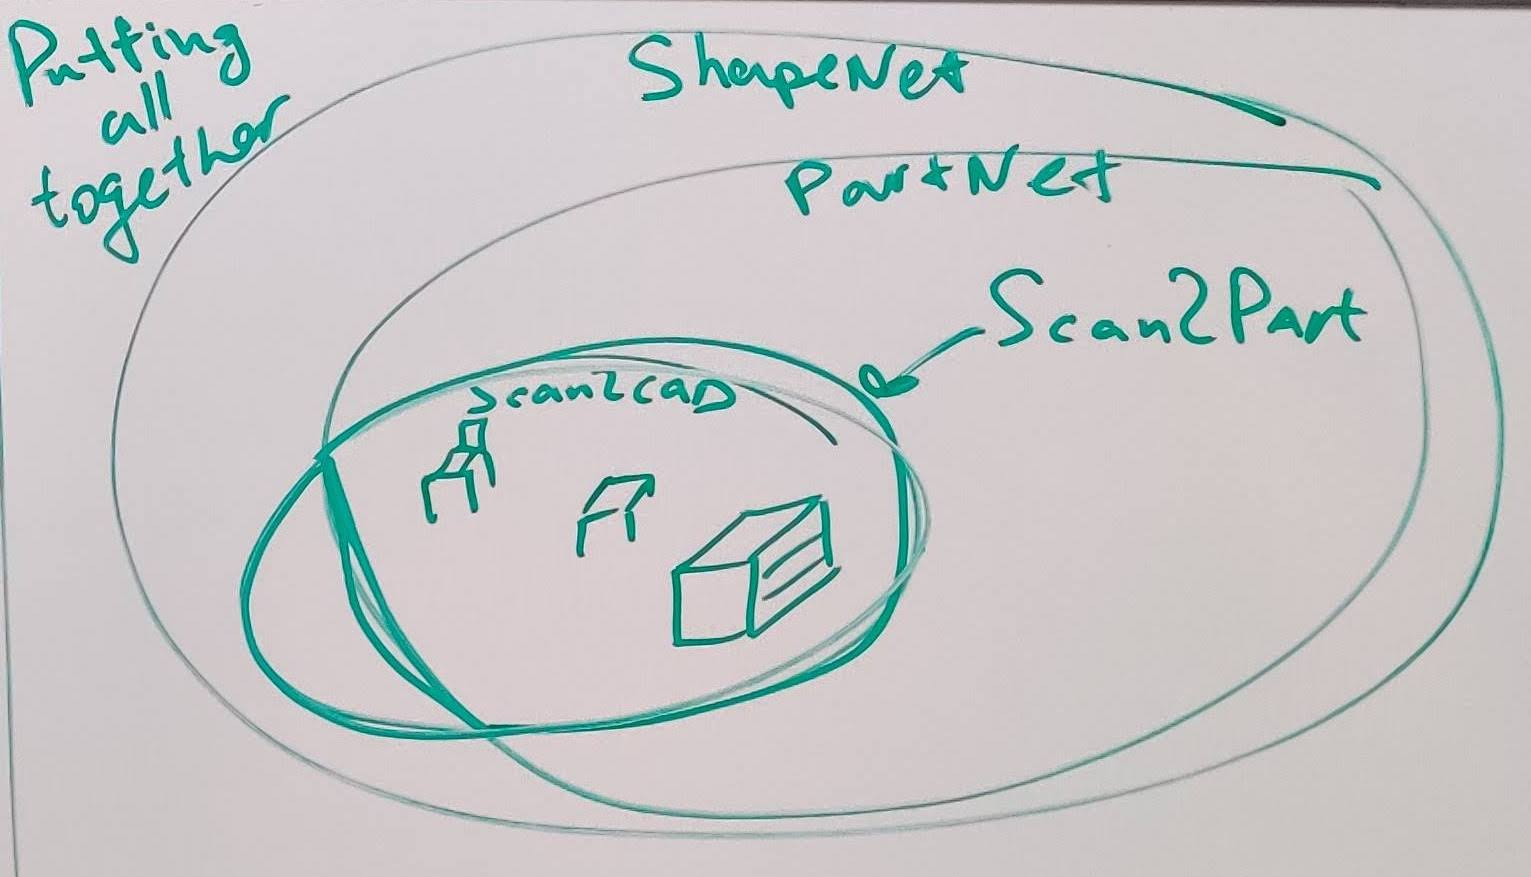
\includegraphics[trim=0 0 0 0, max width=0.5\textwidth]{Figures/scan2part/dataset_overlap.jpg}
% \caption{Venn Diagram of Datasets (PartNet $\subset$ Shapenet, Scan2CAD $\subset$  Shapenet)}
% \end{figure}

% \subsection{Labeling}
% \subsubsection{Shapenet to PartNet}
% \textbf{Projection}
% % \caption{left picture: gray shapenet, right picture: colored partnet}
% \textbf{ICP} 
% % \caption{two histogram of AVG CD between two objects: before and after ICP}
% % \caption{best and worst cases according to previous histogram}
% \subsubsection{Scan2CAD: ScanNet to Shapenet}
% % \caption{example from the Scan2CAD dataset}
% \subsection{Data-driven part taxonomy}

% After joining instance labels to class labels number of elements is reduced first to 53k, then to 20k, and finally to 308 classes.

% After further pruning because 20 of the part classes don't have a single voxel, number of classes can be reduced from 308 to 288 classes.
% % \caption{histogram of voxel appearance on the scenes}
% % \caption{example of prunned classes}
% % \caption{example of good class (not so deep)}
% \subsection{Model-driven part taxonomy}

% \subsection{Scan2Part}
% % \caption{tiser}

% \begin{table}[]
% \centering
% \caption{Dataset funnels}
% \label{tab:dataset_funnels}
% \begin{tabular}{l|l|l|l|l}
%  & Total count & PartNet & Scan2CAD & Scan2Part \\
% \hline
% Scenes from ScanNet & 1.5k & - & 1.5k & 1.5k \\
% Shapes from ShapeNet & 30k & 24k & 3k & 2.7k
% \end{tabular}
% \end{table}

% \begin{figure}
% \label{fig:Partnet_overview}
%   \centering
% % 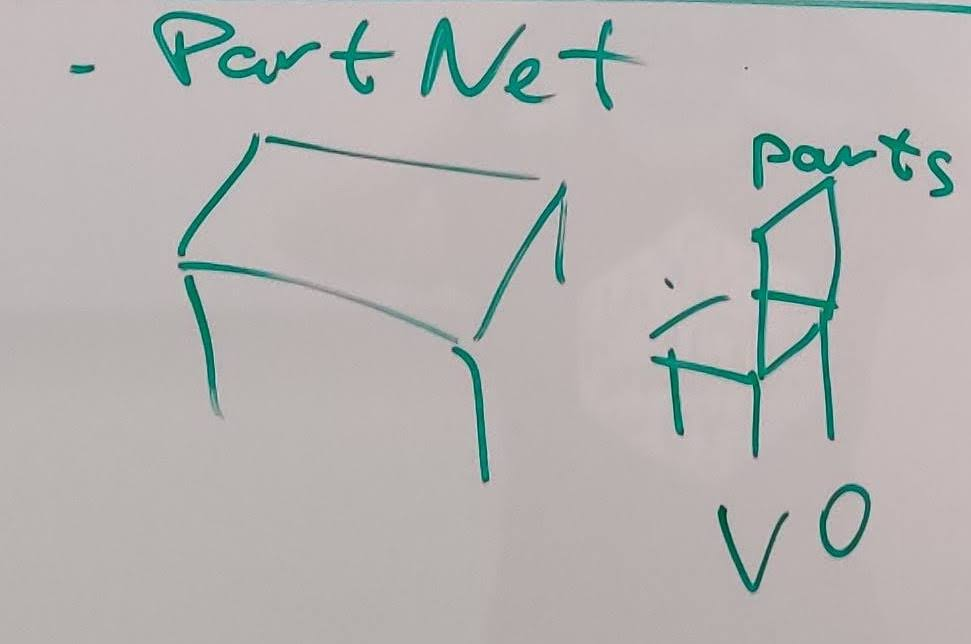
\includegraphics[trim=0 0 0 0, max width=0.5\textwidth, right]{Figures/scan2part/Partnet_overview.jpg}
% 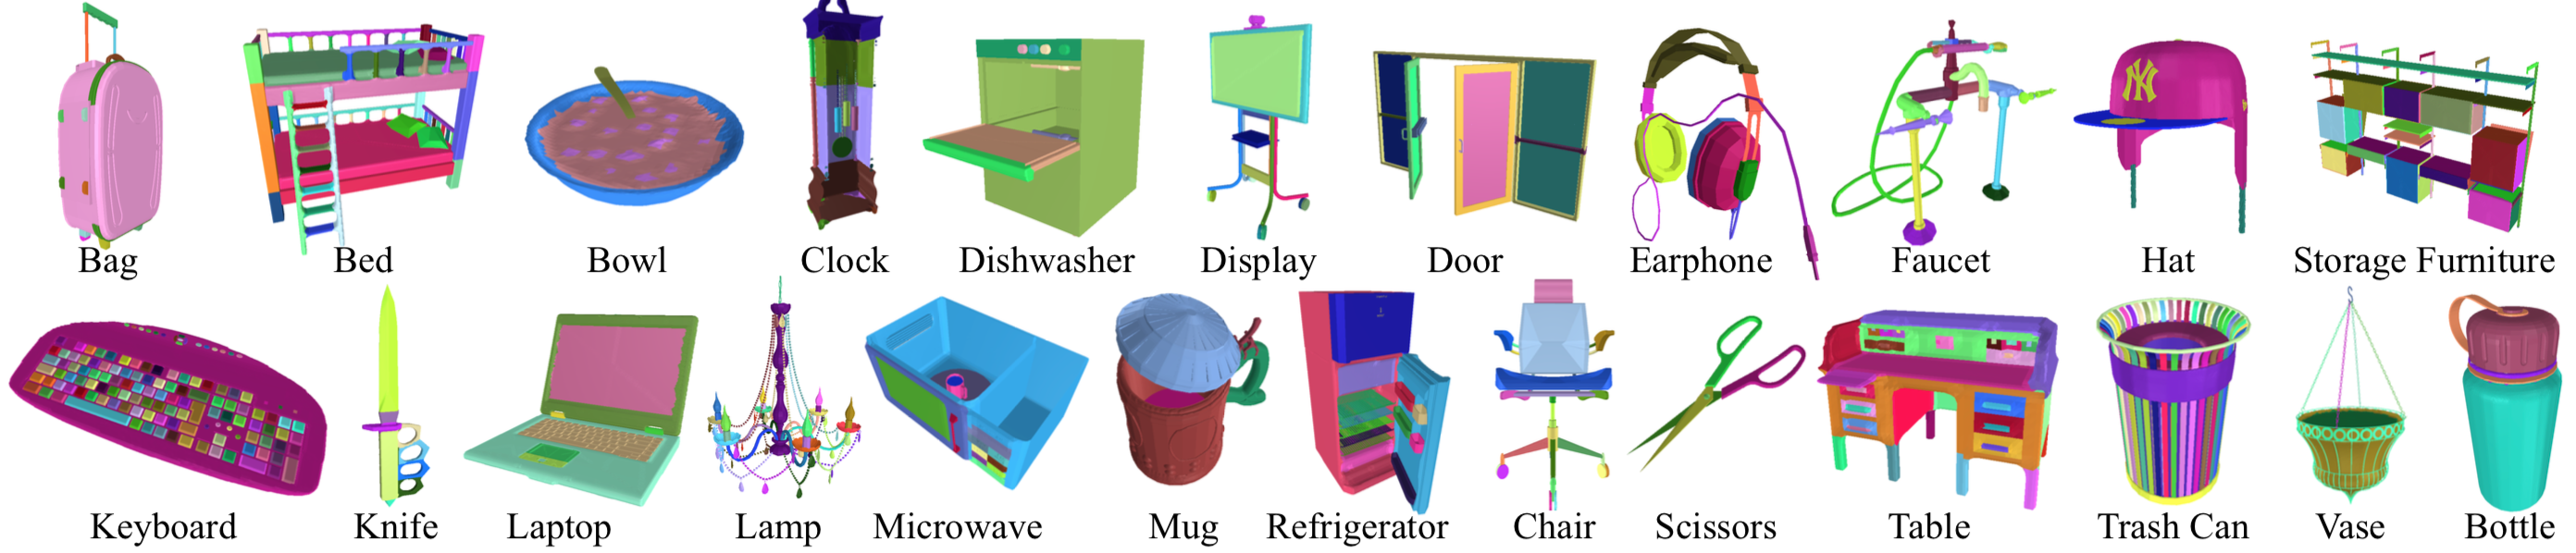
\includegraphics[trim=0 0 0 0, max width=\textwidth, right]{Scan2Part/images/partnet_data_visu.png}
% \caption{Partnet overview}
% \end{figure}

% В изображении~\ref{fig:partnet_to_scannet_labeling}а можно увидеть различие в детальности полигональной сетки в объектах датасетов ShapeNet и PartNet, высокая полигональность - последствие метода разметки деталей объекта в web-интерфейсе.
% На графике~\ref{fig:partnet_to_scannet_labeling}б изображено расспределение метрики Чамфера на соответствующих объектах в датасетах ShapeNet и PartNet, как можно заметить многие формы объектов в своих исходных положениях отличаются значительно. Поэтому для установления общей системы координат требуется решить задачу регистрации, которую мы решаем с помощью метода ICP~\cite{besl1992method}. На графике~\ref{fig:partnet_to_scannet_labeling}в можно увидеть как изменилось расспределние метрики Чамфера, ее высокое значение в некоторых случаях объясняется как нахождение методом ICP локального минимум соответствующему одному из симметричных положений объекта в разных датасетах, и не должно значительно повлиять на перенос разметки в датасет ShapeNet.  

% \clearpage

% % \begin{wrapfigure}{l}{0.25\textwidth}


% \begin{figure}[!htb]
% \label{fig:taxonomy_overview}
% \centering
% 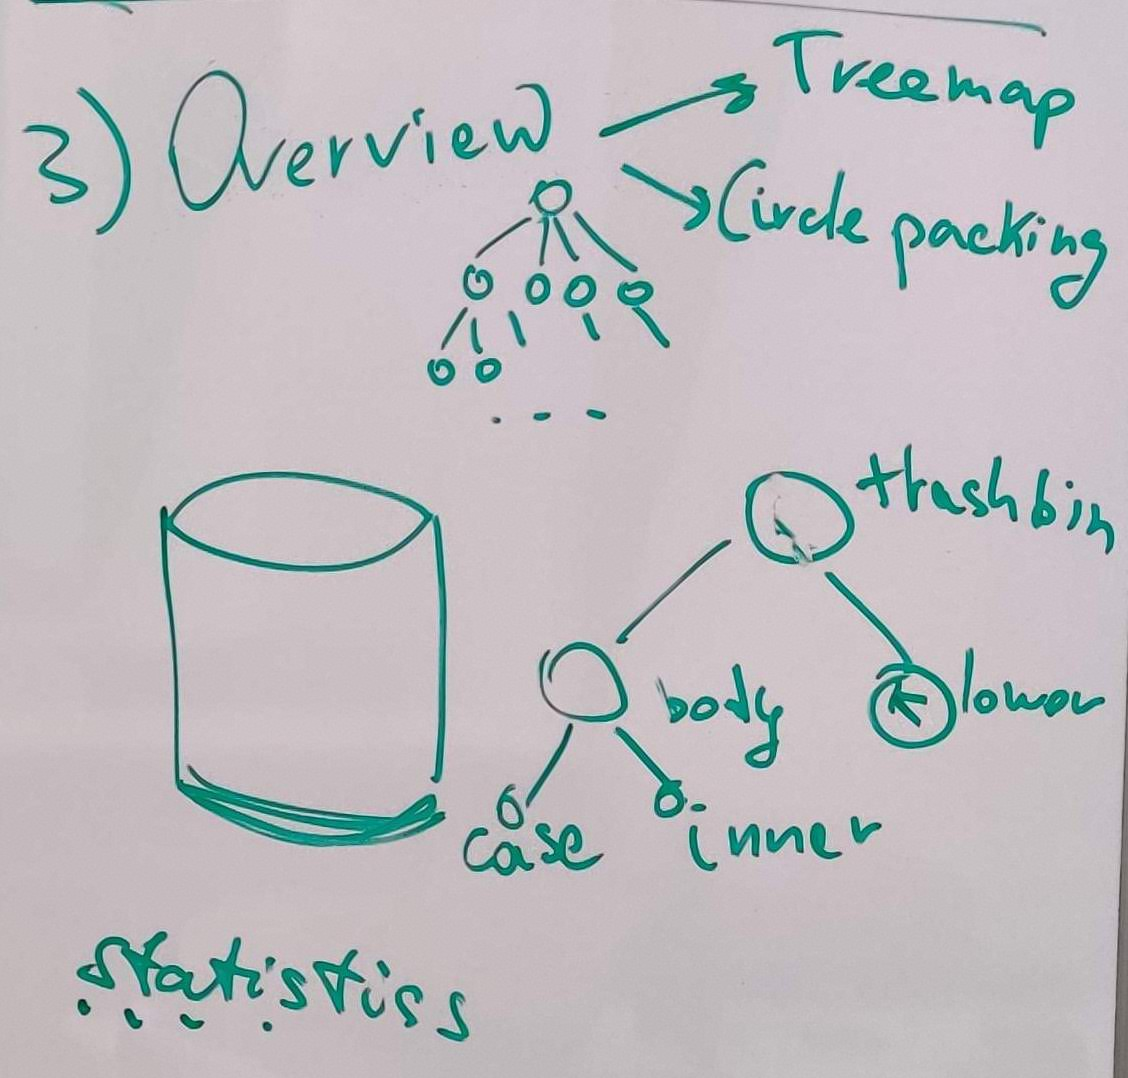
\includegraphics[trim=0 0 0 0, max width=0.5\textwidth]{Figures/scan2part/taxonomy_overview.jpg}
% \caption{taxonomy overview}
% \end{figure}


% \begin{figure}[!htb]
% \label{fig:scan2part_overview}
%   \centering
% 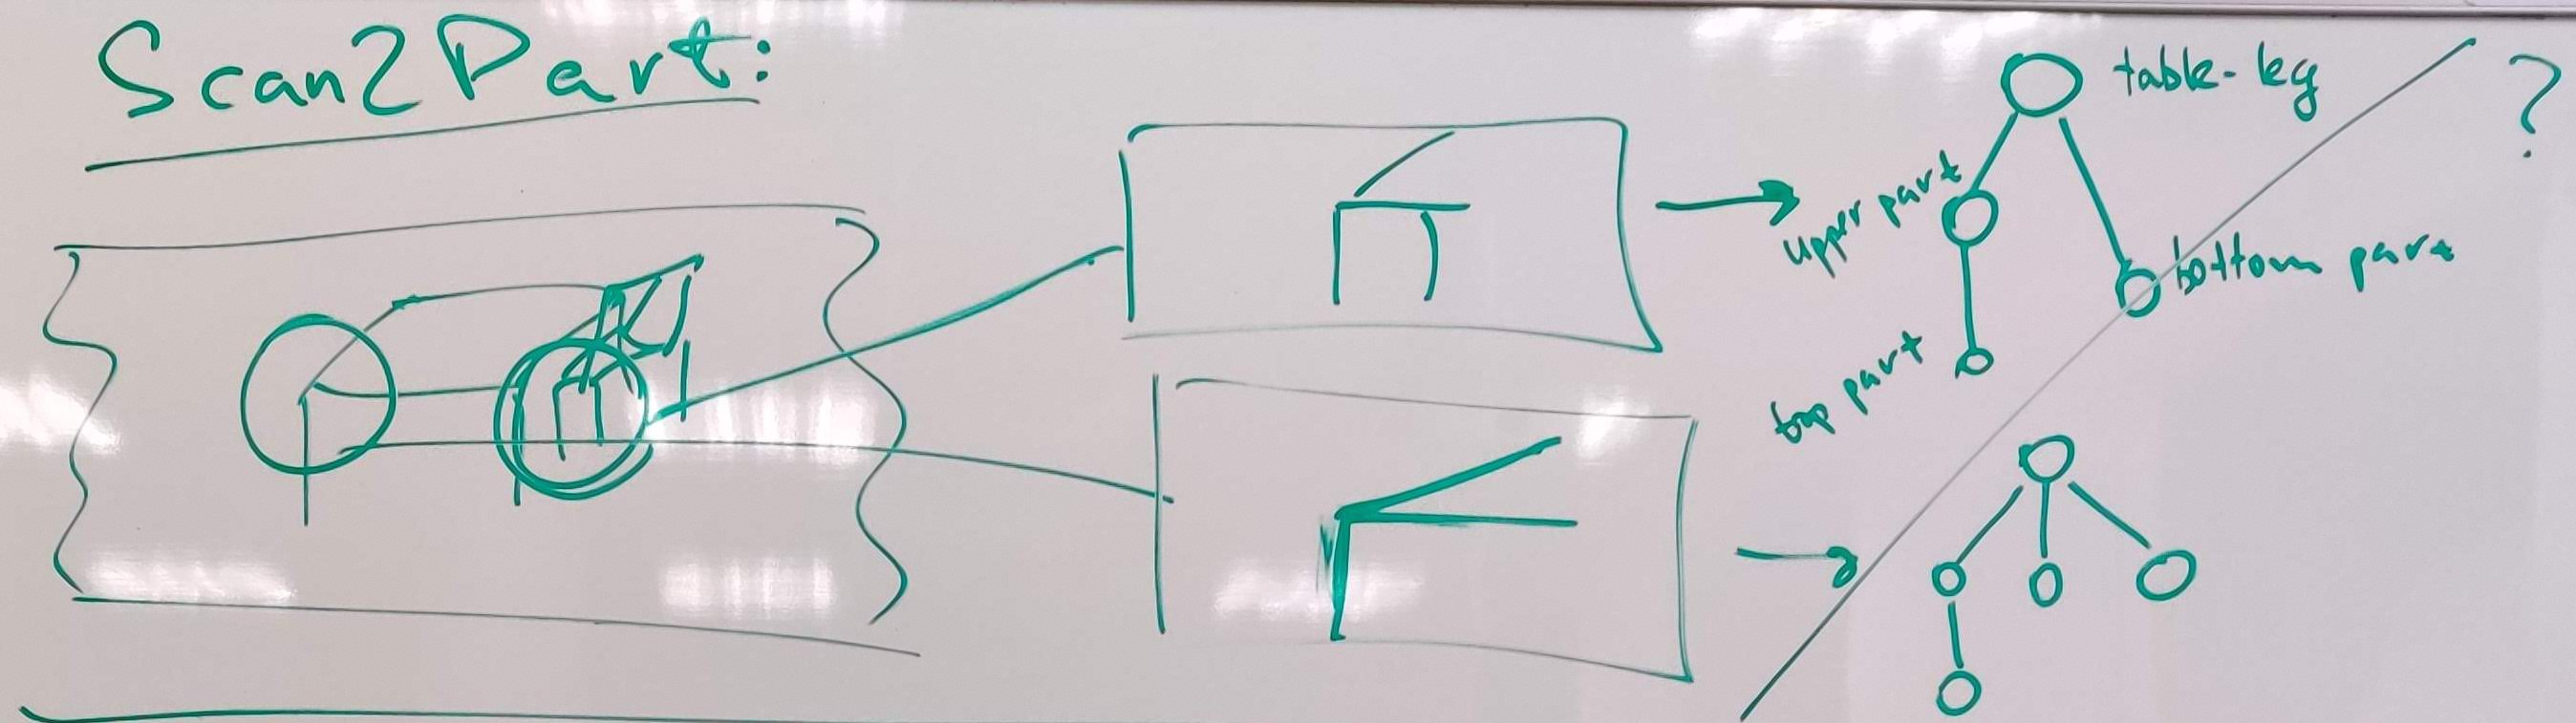
\includegraphics[trim=0 0 0 0, max width=0.5\textwidth]{Figures/scan2part/scan2part_overview.jpg}
% \caption{scan2part overview}
% \end{figure}
% \begin{figure}
% \label{fig:taxonomy_compression}
%   \centering
% 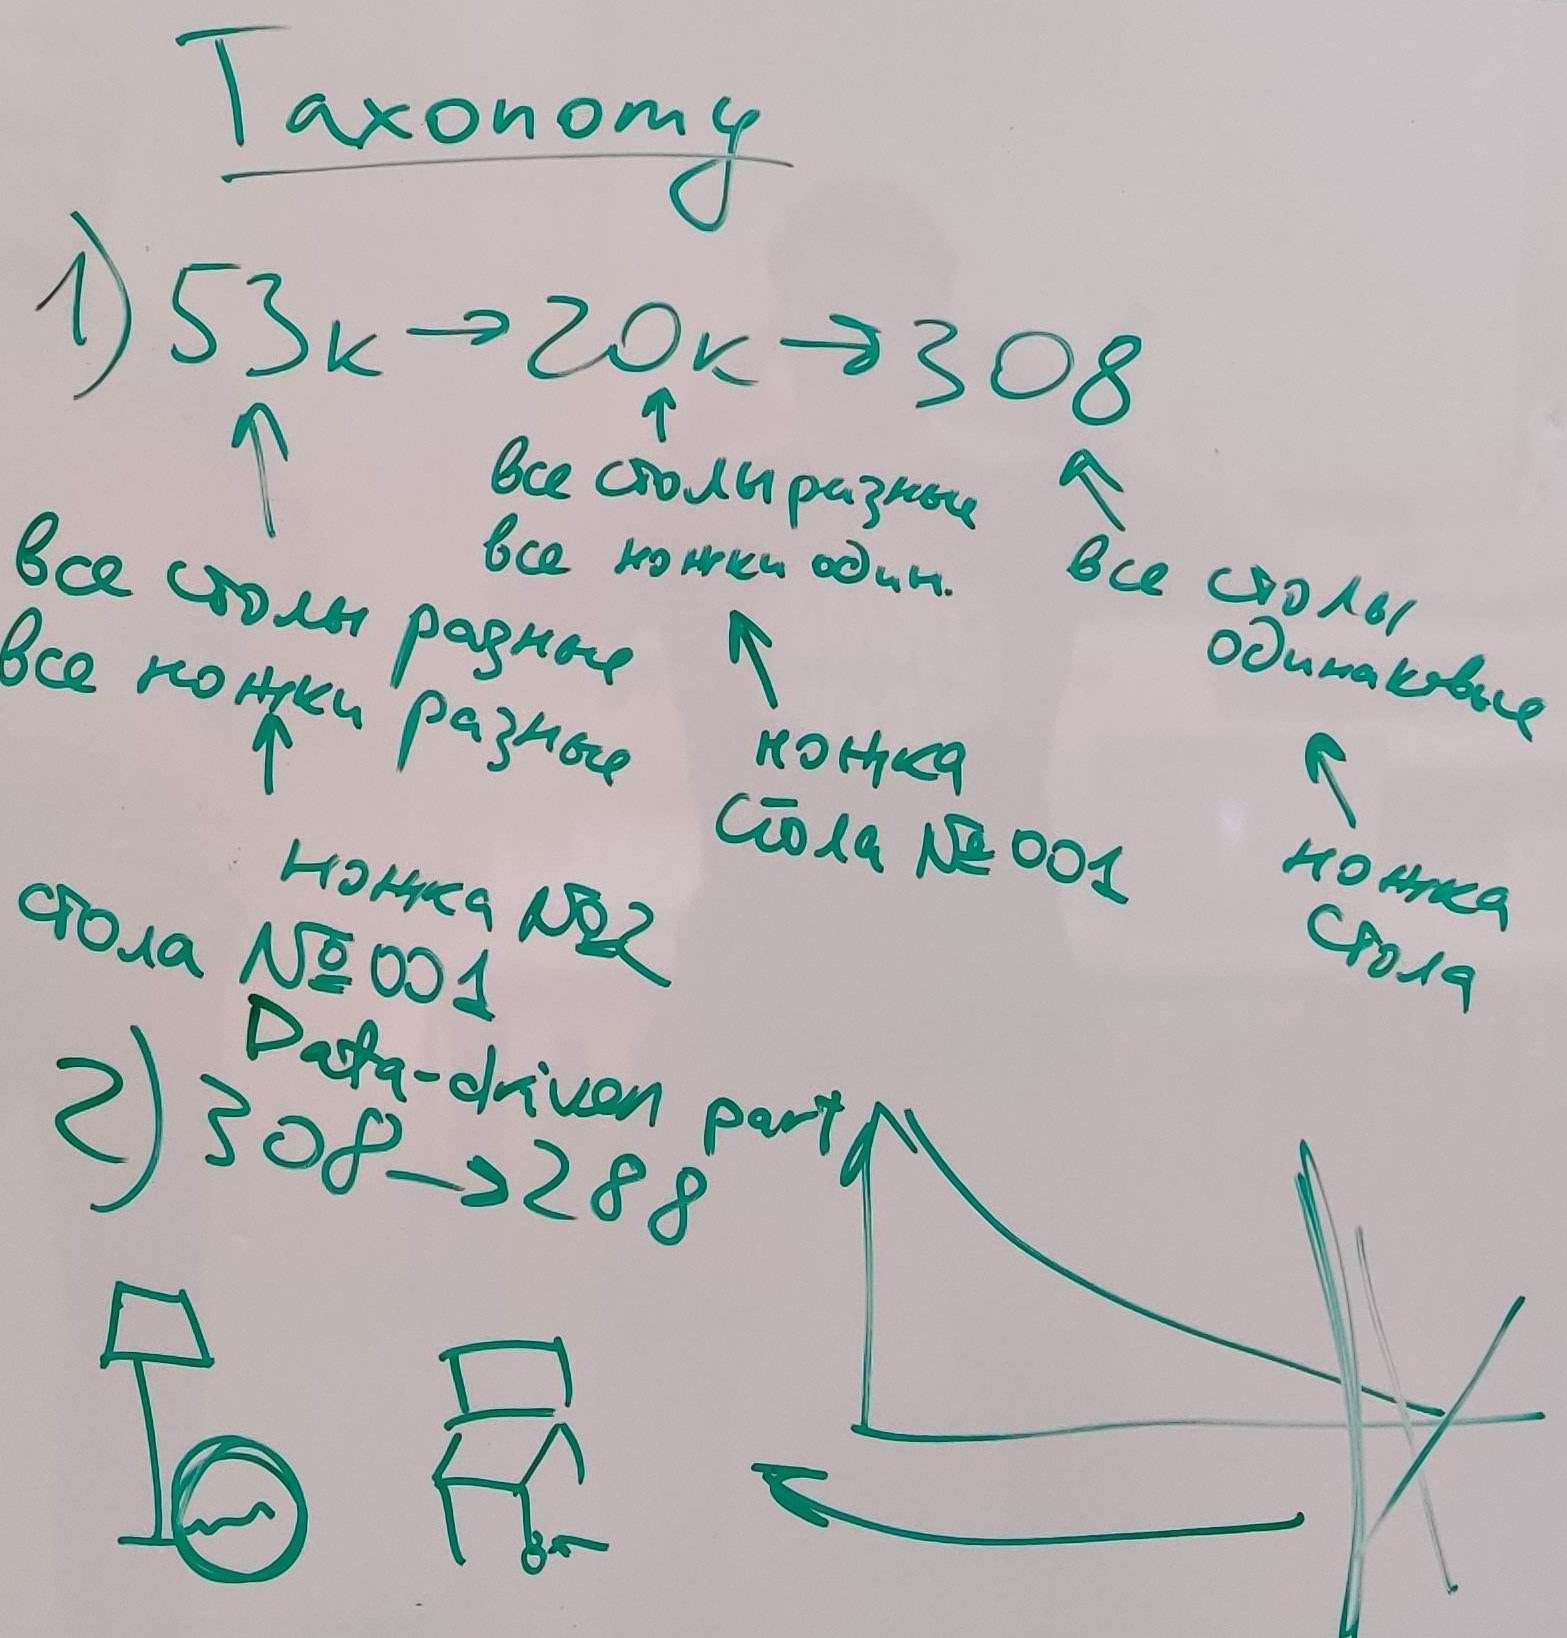
\includegraphics[trim=0 0 0 0, max width=0.5\textwidth]{Figures/scan2part/taxonomy_compression.jpg}
% \caption{taxonomy compression}
% \end{figure}

% \begin{figure}[!htb]
% \label{fig:dataset_mapping}
%   \centering
% 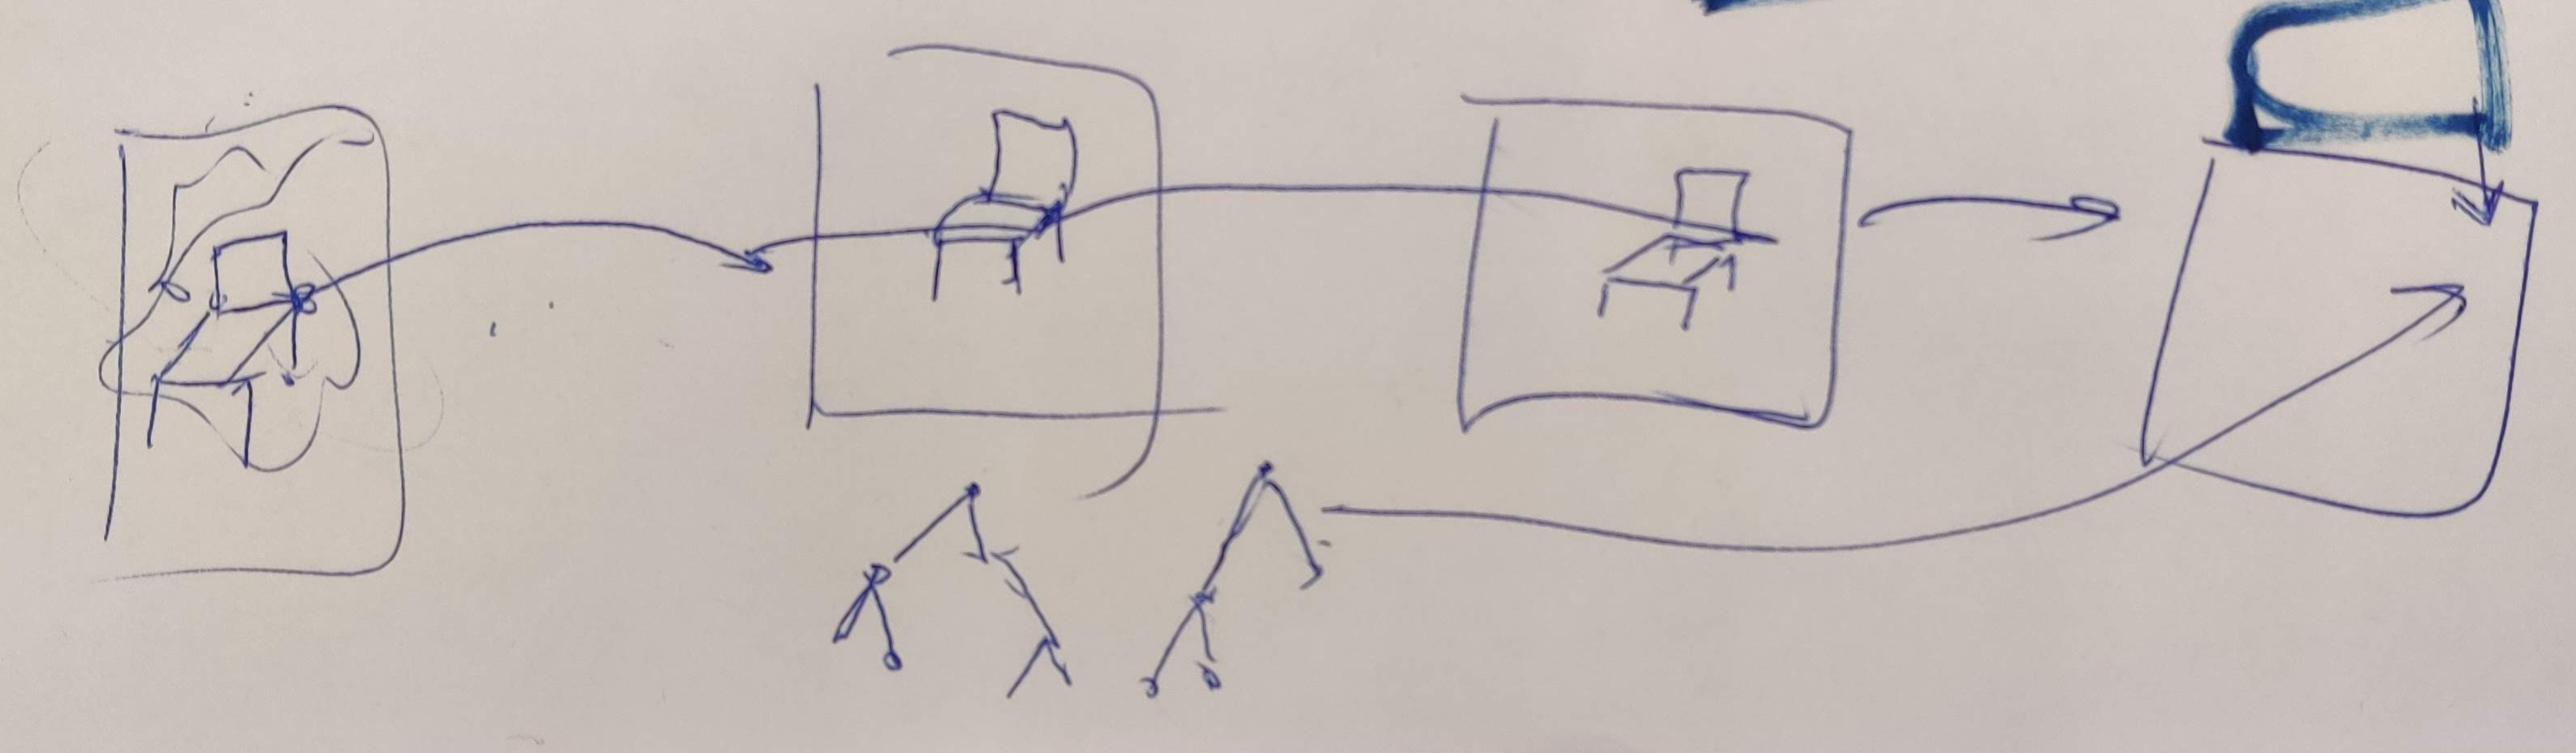
\includegraphics[trim=0 0 0 0, max width=\textwidth]{Figures/scan2part/dataset_mapping.png}
% \caption{Mapping of voxels in ScanNet scene to CAD model and to part hierarchy of the object}
% \end{figure}


% % \subsection{Scan2Part dataset preparation}
% The ScanNet \cite{dai2017scannet} is a dataset of RGB-D scans of real-world indoor scenes with multiple kinds of data representation and semantic object-level labels for those scans.
% The Scan2CAD \cite{avetisyan2019scan2cad} is a dataset that alignes CAD objects from ShapeNet \cite{chang2015shapenet} database to scenes from Scannet, therefore serving as a connective tissue to labels.
% The PartNet \cite{mo2019partnet} is a hierarchical instance level parts dataset of labeles for subset of ShapeNet database. The PartNet dataset the only dataset that has deep hierarchical structure compared to other part annotation datasets like in \cite{Yi16}.

% Using marching cubes algorithm we obtained a voxelised version of scenes from ScanNet dataset with object type labels and mapping of coordinate systems from ScanNet to ShapeNet, because of that we can calculate position of CAD object parts in the scene coordinate system and calculate relative volume in specific voxels thus projecting part labels on scene. 
% Under closer examination we discovered that most of the parts don't have a unique shape making task of instance segmentation for parts very hard to solve and not necessary for practical scene segmentation task.





% 
% 4) При решении собственно задачи понимания сцены на уровней частей естественно возникает некоторая иерархическая структура разметки. 
% — Выбор таксономии играет решащую роль при сегментации, так как слишком грубые таксономии будут неотличимы от просто сегментации и потому бесполезны, а слишком детальные не реализуются из-за ограничений разрешения и шума. 

% \begin{figure}[!t]
% \label{fig:dataset_teaser}
% \centering
% 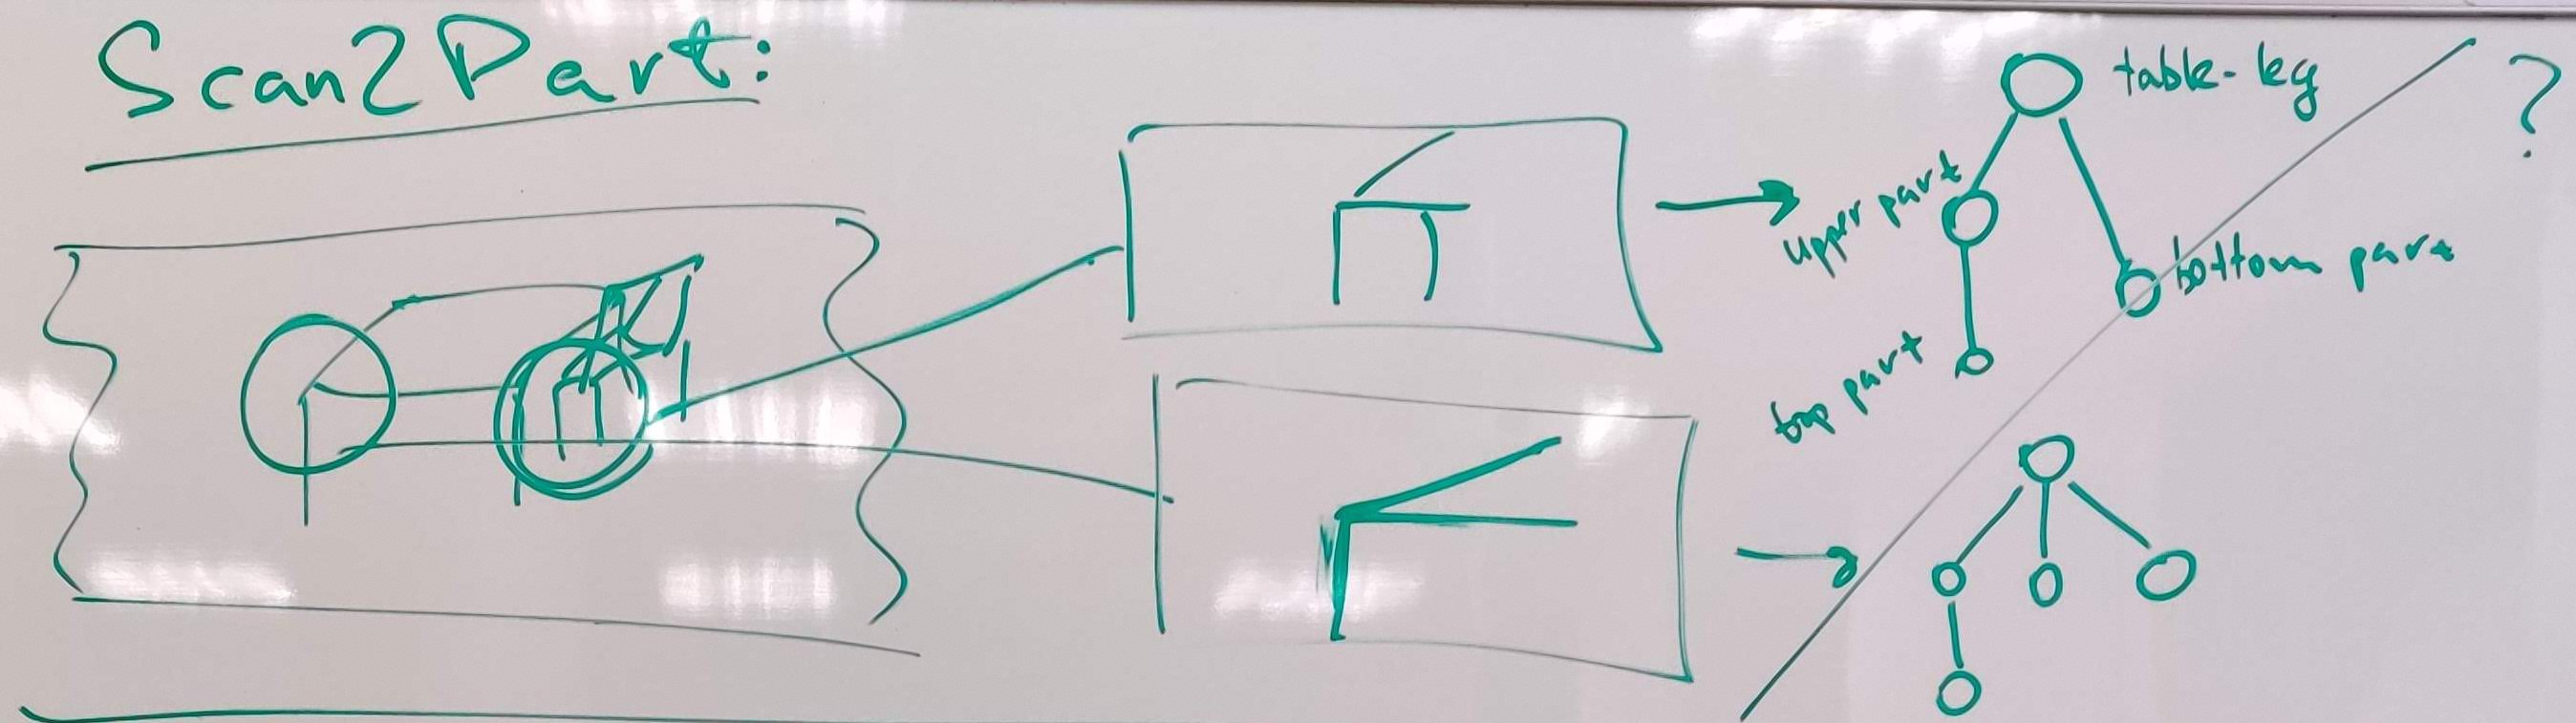
\includegraphics[width=0.9\textwidth]{Figures/scan2part/scan2part_overview.jpg}
% \caption{Dataset teaser}
% \end{figure}

%


% \textcolor{red}{TODO}: Table with abovementioned numbers.

